\documentclass[dvisvgm,border=6mm]{standalone}

\usepackage{tikz}
\usetikzlibrary{arrows.meta, calc, positioning}

\definecolor{dataBlue}{HTML}{1488D8}
\definecolor{modelNavy}{HTML}{030391}
\definecolor{artifactGrey}{HTML}{667085}
\definecolor{inkBlack}{HTML}{101828}

\begin{document}
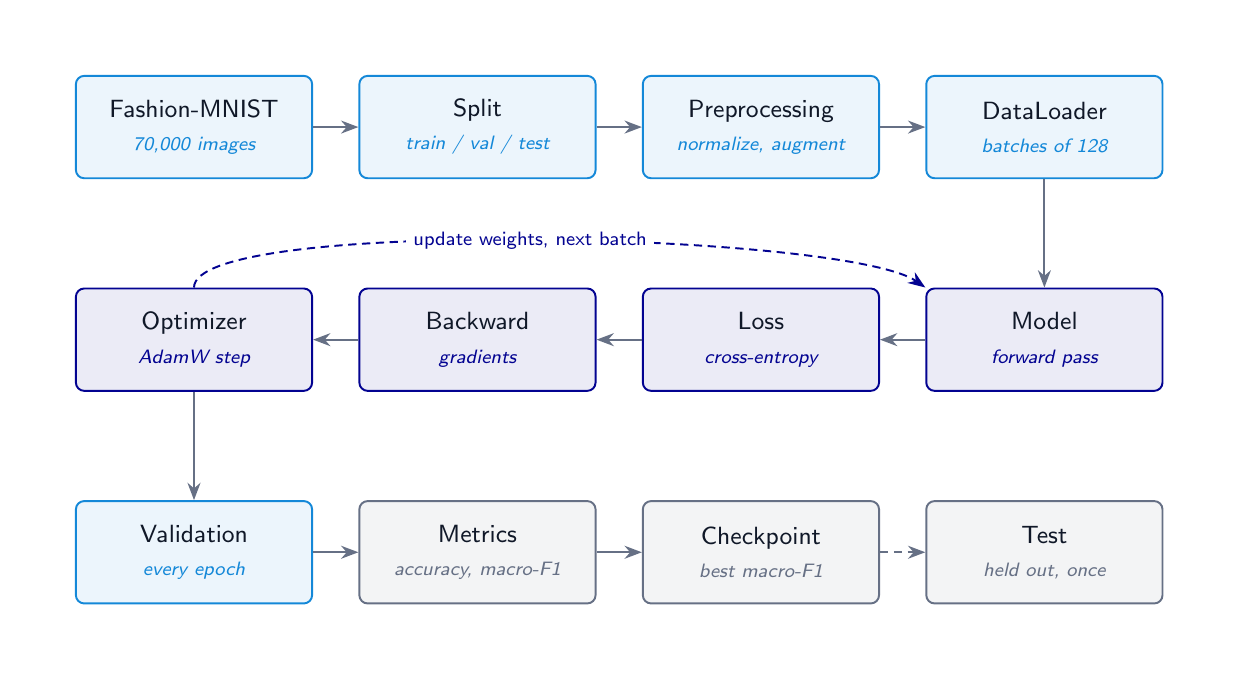
\begin{tikzpicture}[
  font=\sffamily,
  stage/.style={
    rectangle, rounded corners=3pt, draw=#1, line width=0.7pt, fill=#1!8,
    minimum width=30mm, minimum height=13mm, align=center,
    text=inkBlack, font=\sffamily\small, inner sep=3pt,
  },
  sub/.style={font=\sffamily\scriptsize\itshape, text=#1},
  flow/.style={-{Stealth[length=2.2mm]}, draw=artifactGrey, line width=0.7pt},
  feedback/.style={flow, draw=modelNavy, densely dashed},
  held/.style={flow, densely dashed},
  lbl/.style={font=\sffamily\scriptsize, text=#1, inner sep=2pt},
  x=36mm, y=-27mm,
]

\node[stage=dataBlue] at (0,0) (data)   {Fashion-MNIST\\[1pt] \textcolor{dataBlue}{\scriptsize\itshape 70,000 images}};
\node[stage=dataBlue] at (1,0) (split)  {Split\\[1pt] \textcolor{dataBlue}{\scriptsize\itshape train / val / test}};
\node[stage=dataBlue] at (2,0) (prep)   {Preprocessing\\[1pt] \textcolor{dataBlue}{\scriptsize\itshape normalize, augment}};
\node[stage=dataBlue] at (3,0) (loader) {DataLoader\\[1pt] \textcolor{dataBlue}{\scriptsize\itshape batches of 128}};

% training loop, right to left
\node[stage=modelNavy] at (3,1) (model) {Model\\[1pt] \textcolor{modelNavy}{\scriptsize\itshape forward pass}};
\node[stage=modelNavy] at (2,1) (loss)  {Loss\\[1pt] \textcolor{modelNavy}{\scriptsize\itshape cross-entropy}};
\node[stage=modelNavy] at (1,1) (grad)  {Backward\\[1pt] \textcolor{modelNavy}{\scriptsize\itshape gradients}};
\node[stage=modelNavy] at (0,1) (opt)   {Optimizer\\[1pt] \textcolor{modelNavy}{\scriptsize\itshape AdamW step}};

\node[stage=dataBlue]     at (0,2) (valid)  {Validation\\[1pt] \textcolor{dataBlue}{\scriptsize\itshape every epoch}};
\node[stage=artifactGrey] at (1,2) (metric) {Metrics\\[1pt] \textcolor{artifactGrey}{\scriptsize\itshape accuracy, macro-F1}};
\node[stage=artifactGrey] at (2,2) (ckpt)   {Checkpoint\\[1pt] \textcolor{artifactGrey}{\scriptsize\itshape best macro-F1}};
\node[stage=artifactGrey] at (3,2) (test)   {Test\\[1pt] \textcolor{artifactGrey}{\scriptsize\itshape held out, once}};

\draw[flow] (data)   -- (split);
\draw[flow] (split)  -- (prep);
\draw[flow] (prep)   -- (loader);
\draw[flow] (loader) -- (model);
\draw[flow] (model)  -- (loss);
\draw[flow] (loss)   -- (grad);
\draw[flow] (grad)   -- (opt);

\draw[feedback] (opt.north) .. controls +(0,9mm) and +(-10mm,7mm) .. (model.north west)
  node[lbl=modelNavy, midway, fill=white, inner sep=2.5pt] {update weights, next batch};

\draw[flow] (opt) -- (valid);
\draw[flow] (valid)  -- (metric);
\draw[flow] (metric) -- (ckpt);
\draw[held] (ckpt)   -- (test);

\path (current bounding box.north west) ++(-6mm,6mm)
      (current bounding box.south east) ++(6mm,-6mm);

\end{tikzpicture}
\end{document}
